% (C) 2016 Jean Nassar. Some Rights Reserved
% Except where otherwise noted, this work is licensed under the Creative Commons Attribution-ShareAlike License, version 4
% Experiments
% \chapter{Experiments}
% \label{ch:experiments}
\chapter{Experiment Design}
%\epigraphhead{\epigraph{
%There is no such thing as a failed experiment, only experiments with unexpected outcomes.}{\textsc{Richard Buckminster Fuller}}}

\section{Objectives}
  The experiments were conducted in order to evaluate the efficiency and efficacy of \gls{spirit} with respect to a conventional onboard camera in an environment with low communication bandwidth.
  These were evaluated using both objective and subjective measures, as described in Section \ref{sec:experiment_eval}.
  Particularly of interest were the spacial accuracy with respect to a target, and the time required to complete the task.

\section{Participants}
A total of nine people participated in the study.
All were volunteers, male, and students of Kyoto University.
The youngest was 22\,years old, and the oldest was 29.
The mean age was 24.2 years old, and the standard deviation was 2.1 years.

Information was collected about their experiences.
Three had some experience flying teleoperated robots, of which one had some experience with quadcopters.
No participants had any other flying experience, including flight simulators.

An information pamphlet was prepared, and written consent was obtained from each in order to comply with ethical obligations.

\begin{wrapfigure}{r}{0.47\textwidth}
  \centering
  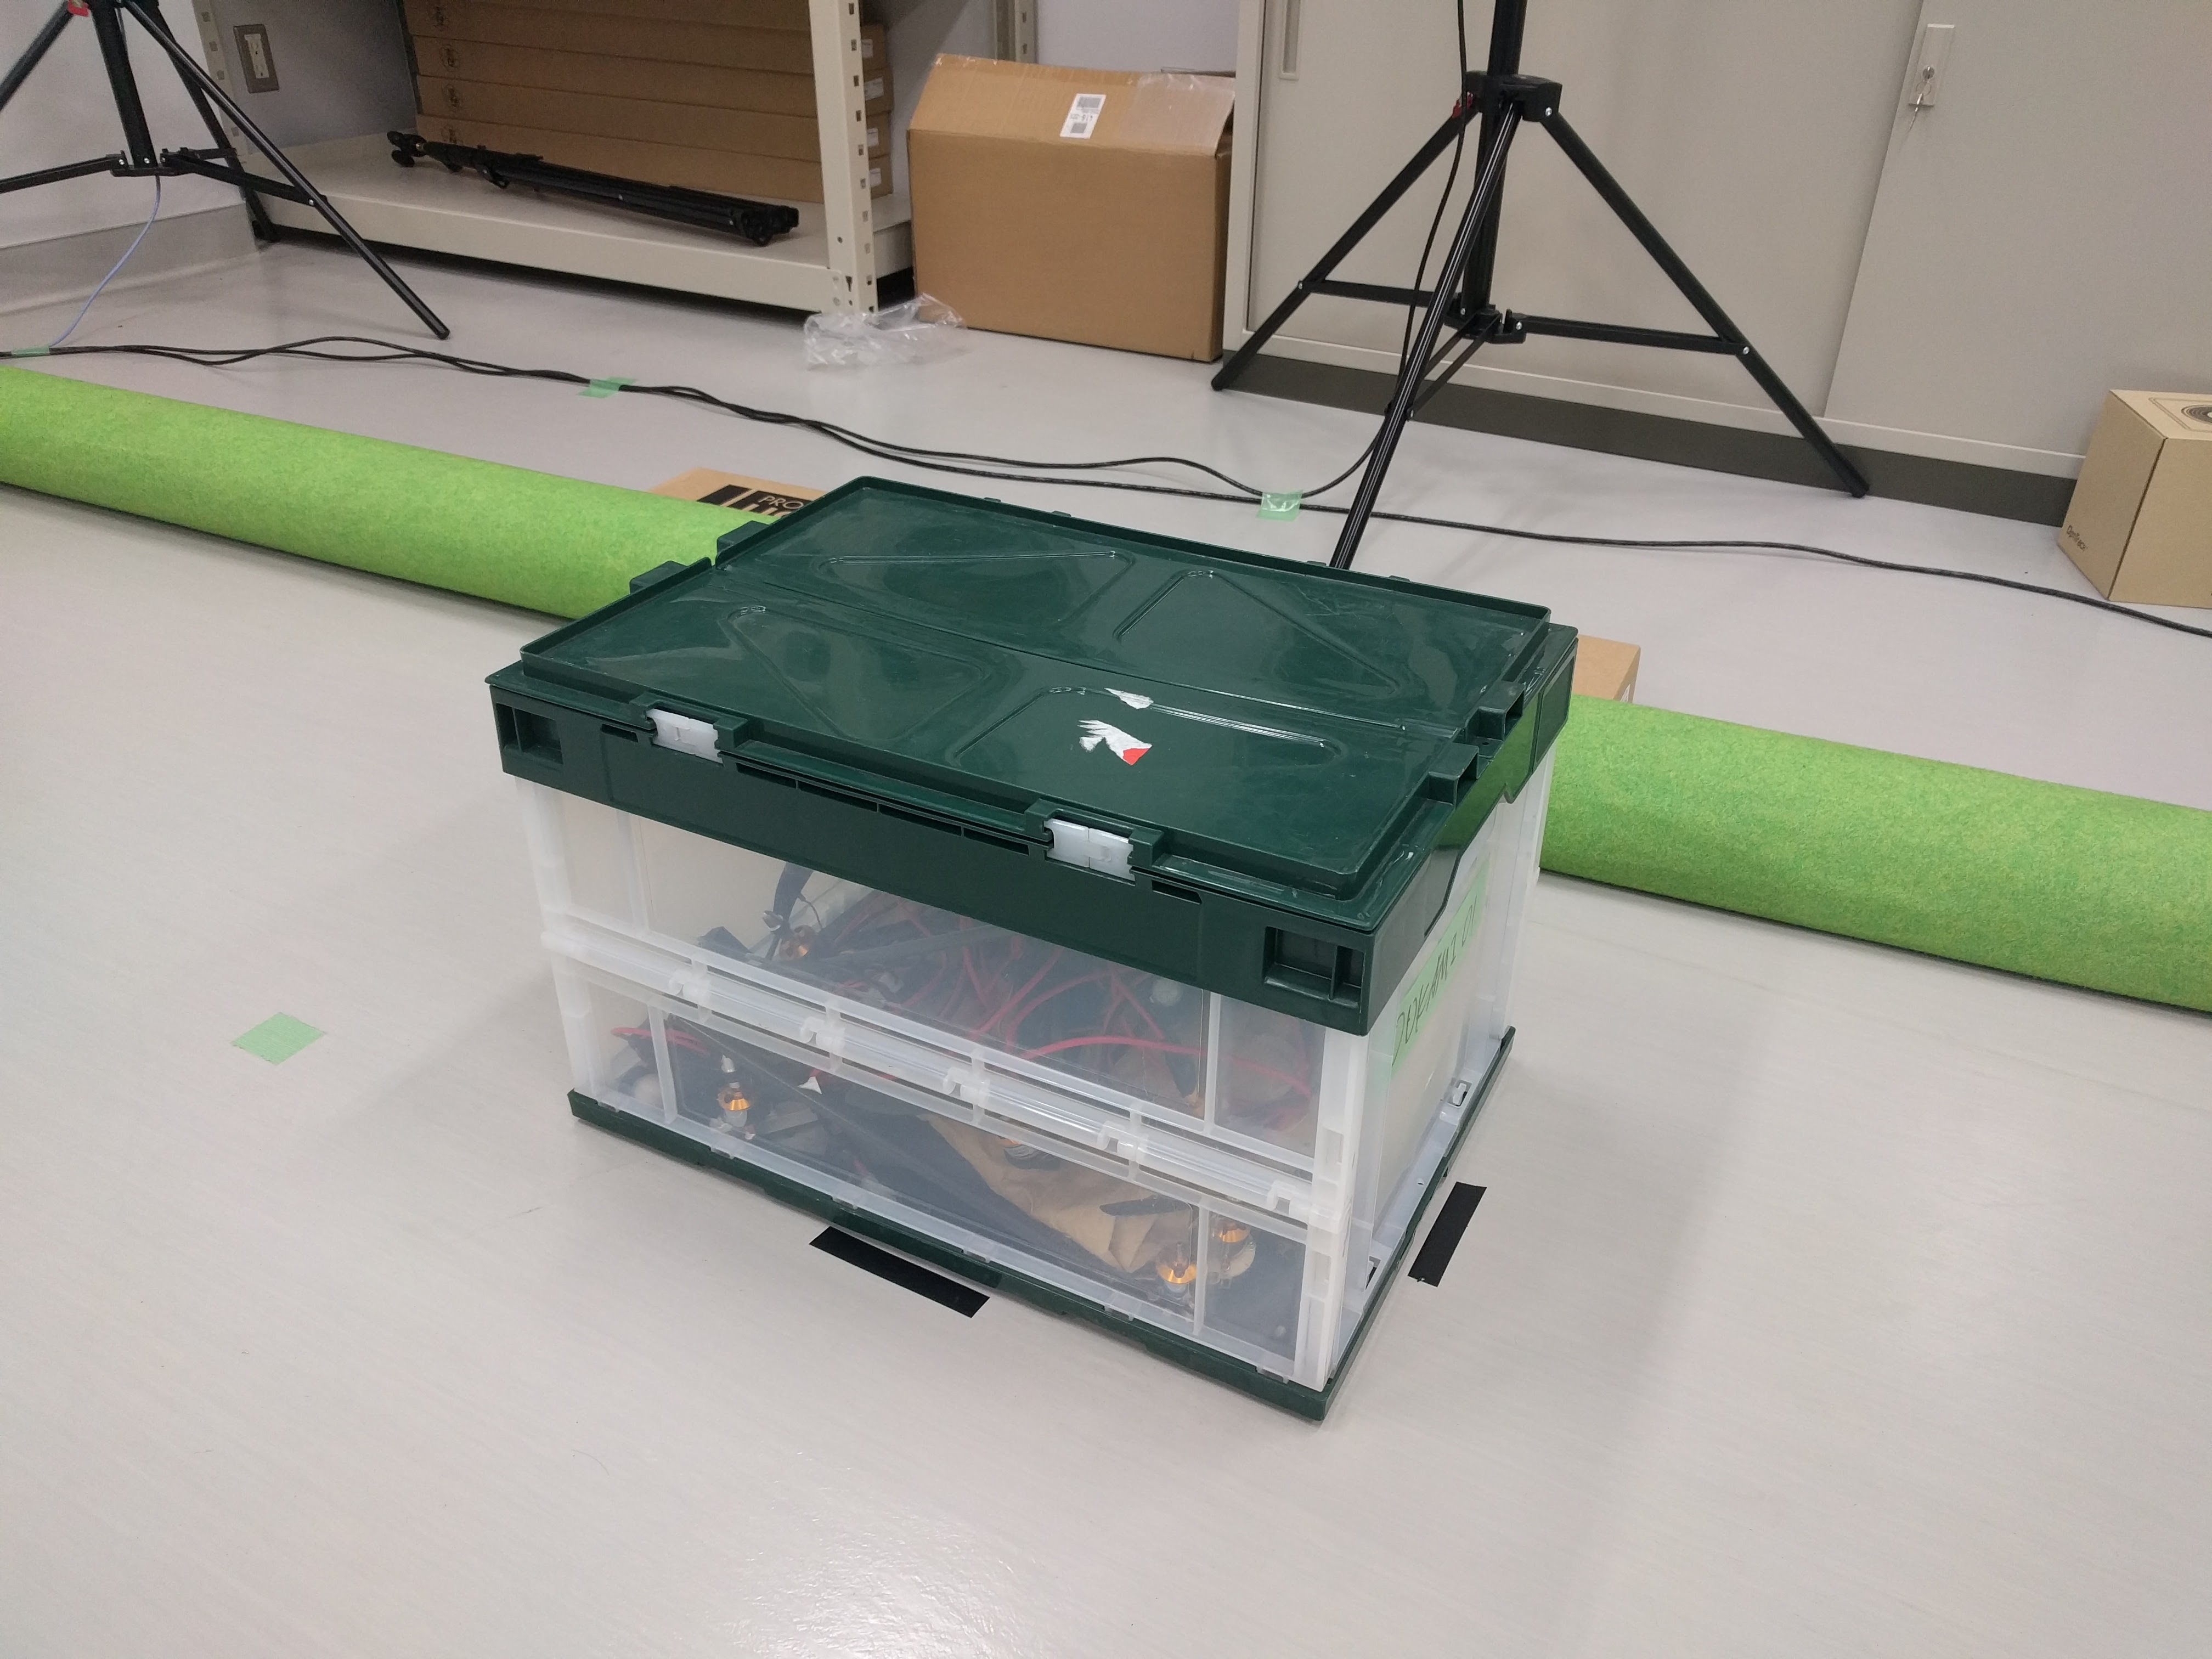
\includegraphics[width=0.45\textwidth]{target}
  \caption[Target]{
    The target which users aim towards.
  }
  \label{fig:target}
\end{wrapfigure}

\section{Experiment setup}
The participants were asked to fly a drone from a starting point to a target 6\,m away.
The target itself (\fref{fig:target}) was a raised box 52.5\,cm wide, 37\,cm deep, and 34\,cm high.
When they believe that they have arrived, they would indicate as much by pressing a button on the controller, before landing safely.
The setup of the flying area can be seen in \fref{fig:flying_area}.

The drone itself was not always stable, and sometimes changed heights or rotated significantly upon takeoff.
As a result, the takeoff pad was visible to the operators to minimize the potential for damage to equipment or injury to others.
The drone would no longer be visible after moving a short distance towards the target.
A closeup of the drone on the launchpad is shown in \fref{fig:drone_long_target}.

\begin{figure}
\centering
\hfill
\begin{minipage}{0.45\textwidth}
  \centering
  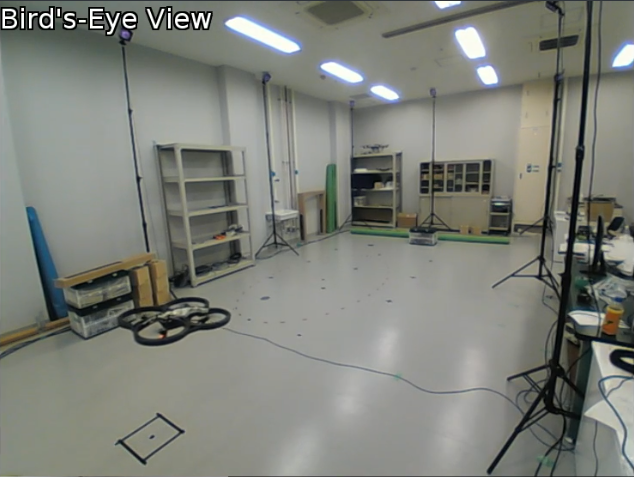
\includegraphics[width=\textwidth]{spirit_flying_area}
  \caption[Flying area]{The flying area which the experiment was set in.}
  \label{fig:flying_area}
\end{minipage}%
\hfill
\begin{minipage}{.45\textwidth}
  \centering
  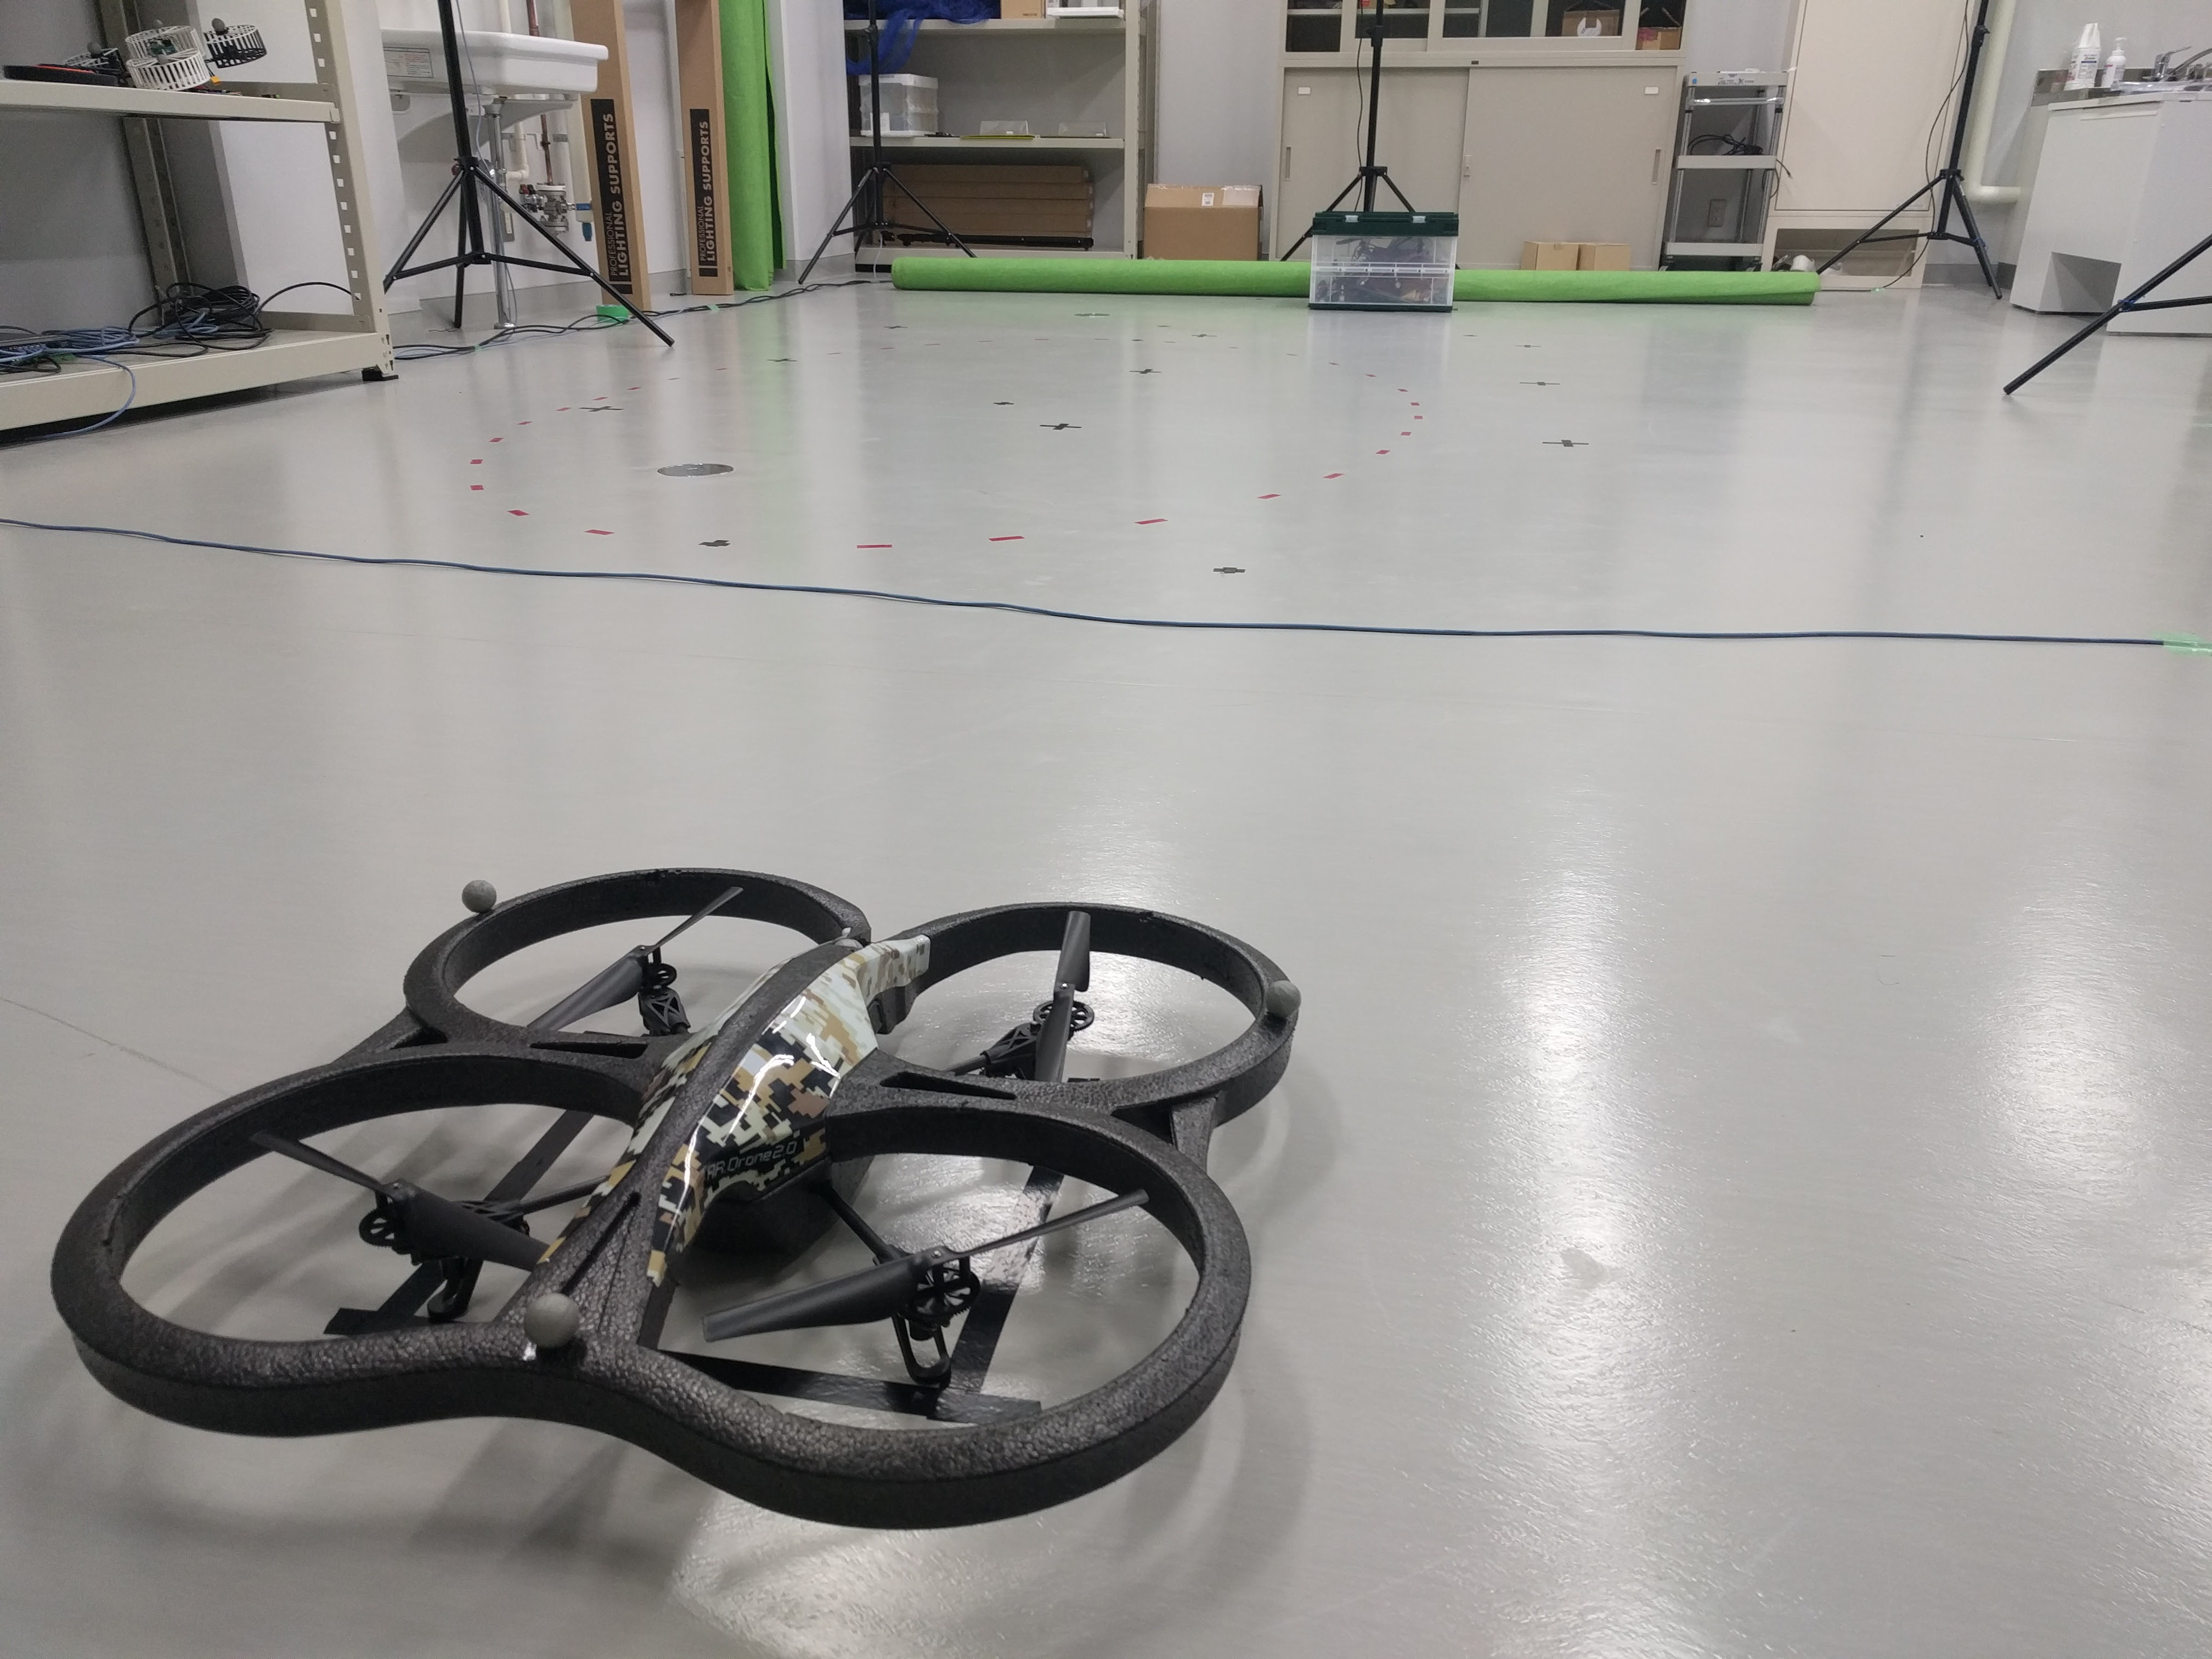
\includegraphics[width=\textwidth]{drone_long_target}
  \caption[Drone on pad]{The drone on the launchpad, looking towards the target.}
  \label{fig:drone_long_target}
\end{minipage}
\hfill
\end{figure}

\subsection{Timeline}
In order to reduce the effect of learning on performance, the order of the trials was changed based on the participant number.
Starting from zero, all five even-numbered participants flew with the onboard view twice before subsequently flying twice with \gls{spirit}.
The four odd-numbered participants started with \gls{spirit}, and then completed the onboard task.

At the beginning of each set of experiments, a verbal explanation was provided to the participant by the experimenter, and consent was obtained.

After that, each user had the opportunity to practice flying the drone for a maximum of five minutes.
This practice could be ended prematurely at the request of the operator.
During practice, both display interfaces were shown at the same time.
There were also no obstructions, so that the user could see the drone all the way to the target, and get a sense of how the correct position and orientation would look like with each system.

After a brief practice session, each person performed one task until the arrival button presses have been received in two runs.
They would then perform the second experiment.
A workload assessments and a survey were completed  after each pair.
Therefore, each subject had four successful runs, and performed two workload assessments and two surveys.
Some performed a larger total number of experiments, but experienced failures usually due to the drone moving up or stopping without user input.
These failures were not considered.

\subsection{Trials}
At the start of each trial, a bird's-eye view and both interface outputs were recorded, and a custom program recorded relevant data to \gls{ros} Bag files.
During any given experiment, the participant was only able to see the relevant interface, while the other was hidden.
A still from one of the recorded videos is shown in \ref{fig:obs}.

\begin{figure}[h]
  \centering
  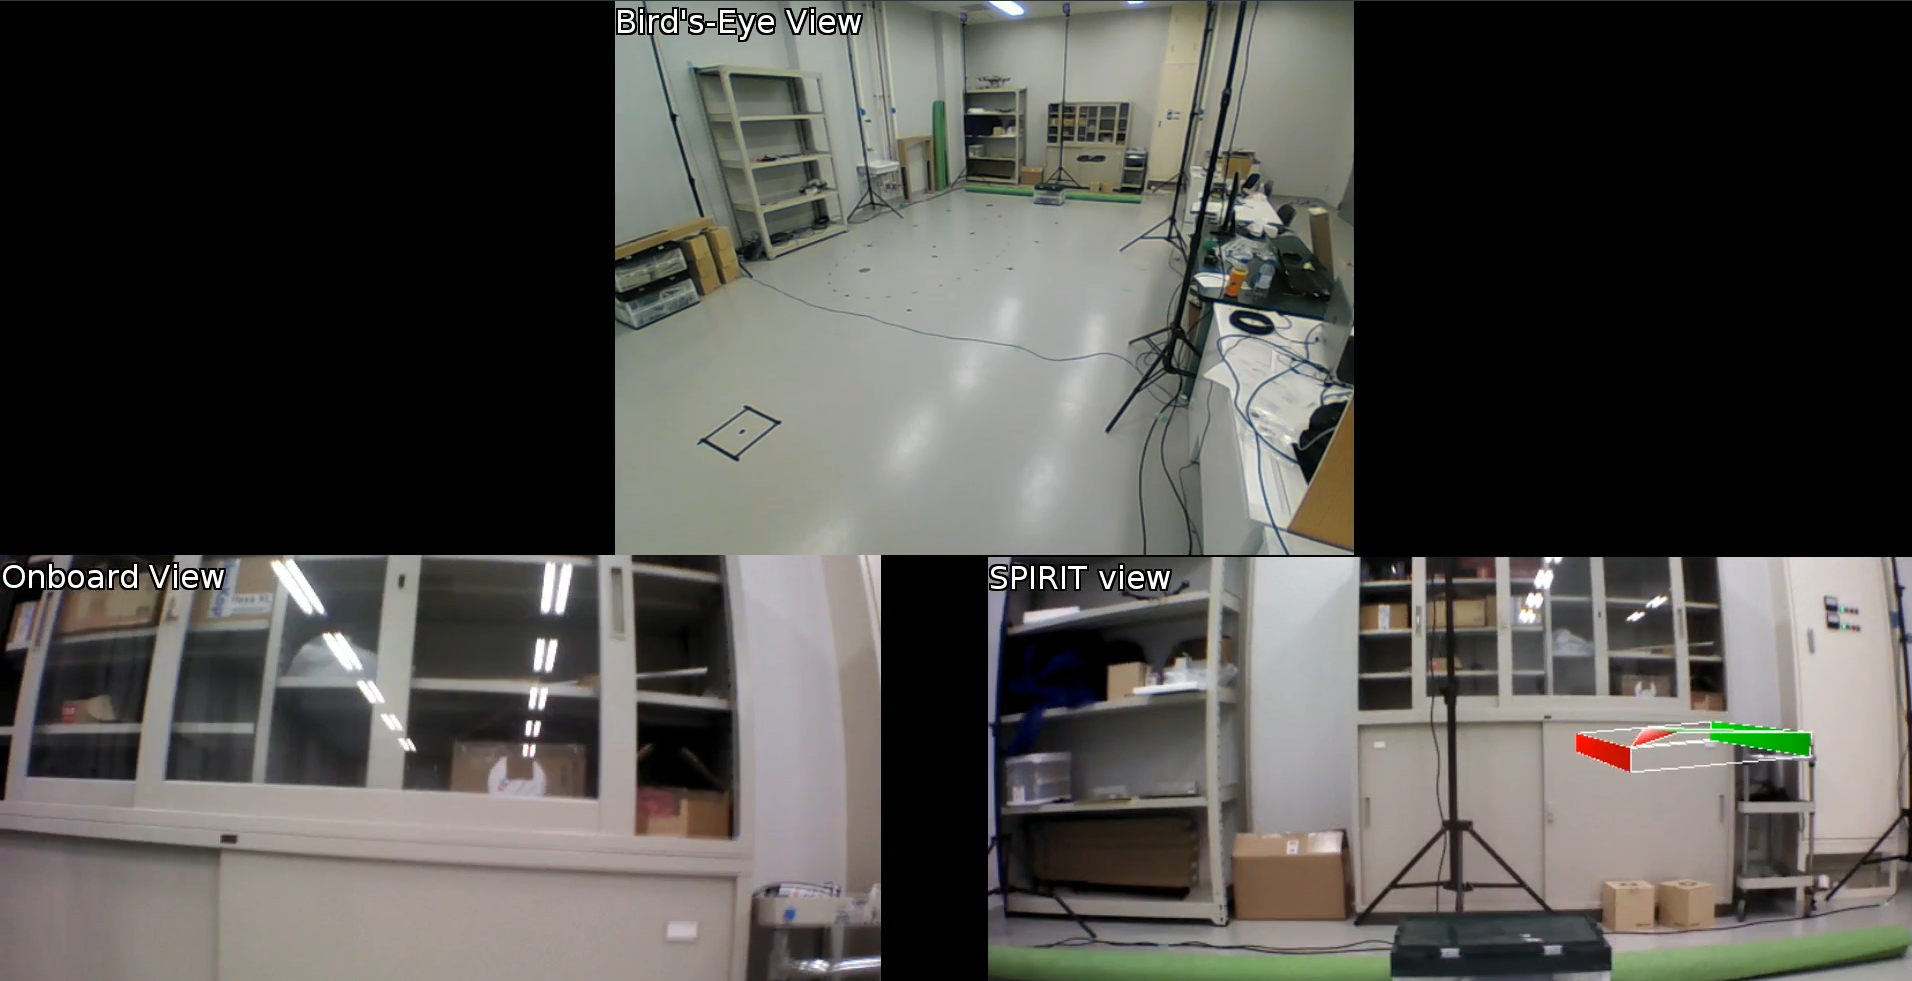
\includegraphics[width=0.9\textwidth]{spirit_recording}
  \caption[Recording sample]{A still from a recorded video.}
  \label{fig:obs}
\end{figure}

Some changes were made to the onboard view to reduce external influences on the results.  
First, while the drone provides video at 30\,Hz, the experiment simulates an area with a bad connection.
The transfer rate was artificially reduced to 2\,Hz, which is the same frequency used by \gls{spirit} to capture frames.
In addition, a loud warning sound used to notify the operator of loss of position tracking was supressed during trials using the onboard view in order to reduce distractions to the operator.

On the other hand for \gls{spirit} trials, no \gls{cg} model was displayed at takeoff because no images had yet been captured of the position.
Upon launch, then, the user would instead move the drone about one body length forward in order to cause the \gls{cg} model to show.
After that, operation would proceed normally until landing.

\section{Evaluation method}
  \label{sec:experiment_eval}
  To analyze the efficiency of the proposed interface, all \gls{ros} topics were recorded and studied.
  The evaluation can be broken down into five groups, as shown below.

  \begin{description}
    \item[Accuracy]
      Accuracy was calculated by using the position of the drone when the arrival button was pressed.
      The data was analyzed by the differences in \sym{posx} and \sym{posy}, as well as the absolute distance from the centre of the target.
    \item[Path length:]
      The path length was calculated by adding the distances between points. Also calculated where the total amount of motion in one axis, and in one direction.
    \item[Duration:]
      Since the amount of time taken from initalization until takeoff varied, the duration of the task was calculated from takeoff to the time of the first arrival button.
    \item[Workload:]
      The self-reported cognitive workload of the operator is measured by using the \gls{nasatlx}, developed by \gls{nasa}.
      Six components are each rated from 0 to 20, inclusive, and then weighted according to their contributions, with a maximum possible score of 100.
      The higher the score, the higher the perceived workload.
    \item[Survey:]
      The participants were asked to complete a survey at the end of each set of tasks, rating their perception on multiple criteria.
      The survey checked control and understanding of position, orientation, and relative position with the target.
      The scale of each question was from 1 to 7, with 7 being the best.

      Free answers were also collected from willing subjects.
  \end{description}

  It was hypothesized that the proposed interface would lead to:

  \begin{itemize}
    \item increased accuracy
    \item shorter path length
    \item shorter duration
    \item lower workload
    \item better user satisfaction
  \end{itemize}
  
\section{Data analysis}
  Since the same people were performing a similar task multiple times, and two repetitions were used for each interface, a repeated measurement design was used.
  
  John K. Kruschke's \gls{best}\cite{kruschke2013} was used in order to evaluate the differences in the physical results obtained from each interface.
  From the paper's abstract:
  
  \begin{quote}
    Bayesian estimation for two groups provides complete distributions of credible values for the effect size, group means and their difference, standard deviations and their difference, and the normality of the data.
    The method handles outliers.
    The decision rule can accept the null value (unlike traditional $t$ tests) when certainty in the estimate is high (unlike Bayesian model comparison using Bayes factors).
    The method also yields precise estimates of statistical power for various research goals.
  \end{quote}

  \gls{best} was implemented in \gls{python} using \gls{pymc3}.
  The sampling algorithm was a Markov Chain Monte Carlo with Metropolis-Hastings.
  2000 steps were calculated.

  The results of \gls{nasatlx} and the survey were analyzed using a paired $t$ test. Because the population size was small, the effect size was calculated using Hedges's \sym{effect}, such that:

  \begin{equation}
    \sym{effect} = \frac{\sym{mean}_1 - \sym{mean}_2}{\sym{std}^\star_\mathrm{pooled}} \times \left(\frac{\sym{popsize} - 3}{\sym{popsize}-2.25}\right) \times \sqrt{\frac{\sym{popsize}-2}{\sym{popsize}}}
  \end{equation}

  \noindent and $\sym{std}^\star_\mathrm{pooled}$, the weighted pooled standard deviation, is:

  \begin{equation}
    \sym{std}^\star_\mathrm{pooled} = \sqrt{\frac{\left(\sym{samplesize}_1-1\right) \sym{std}_1^2 + \left(\sym{samplesize}_2-2\right)\sym{std}_2^2}{\sym{popsize}-2}}
  \end{equation}
